% Gráficos das rodadas de teste fixas (um teste a cada 10 rodadas).
% Pacotes no preâmbulo do documento:
%   \usepackage{pgfplots}
%   \pgfplotsset{compat=1.18}
%
% Convenção visual, igual em todas as figuras de fração de maliciosos:
%   0%  azul, círculo, contínua
%   25% verde, triângulo, contínua
%   50% laranja, quadrado, tracejada
%   65% vermelho, estrela, pontilhada
% Linhas semitransparentes para a sobreposição continuar visível.
% Marcadores só nas rodadas de teste (10, 20, 30, 40, 50).
% Linhas verticais cinza tracejadas marcam essas mesmas rodadas.

\pgfplotsset{
  compat=1.18,
  teste fixo/.style={
    font=\small,
    tick label style={font=\footnotesize},
    label style={font=\small},
    title style={font=\small},
    legend style={
      font=\footnotesize,
      fill=white,
      fill opacity=0.9,
      text opacity=1,
      draw=black!30
    },
    line width=0.9pt,
    xmin=0, xmax=50,
    ymin=0, ymax=1,
    xtick={0,10,20,30,40,50},
    ytick={0,0.2,0.4,0.6,0.8,1},
    xlabel={Rodada},
    grid=major,
    major grid style={black!8},
    clip=false
  }
}
\definecolor{serieZero}{RGB}{31,119,180}
\definecolor{serieVinte}{RGB}{44,160,44}
\definecolor{serieCinquenta}{RGB}{230,120,20}
\definecolor{serieSessenta}{RGB}{200,30,30}
\definecolor{serieMaioria}{RGB}{40,40,40}

\begin{figure}[htbp]
  \centering
  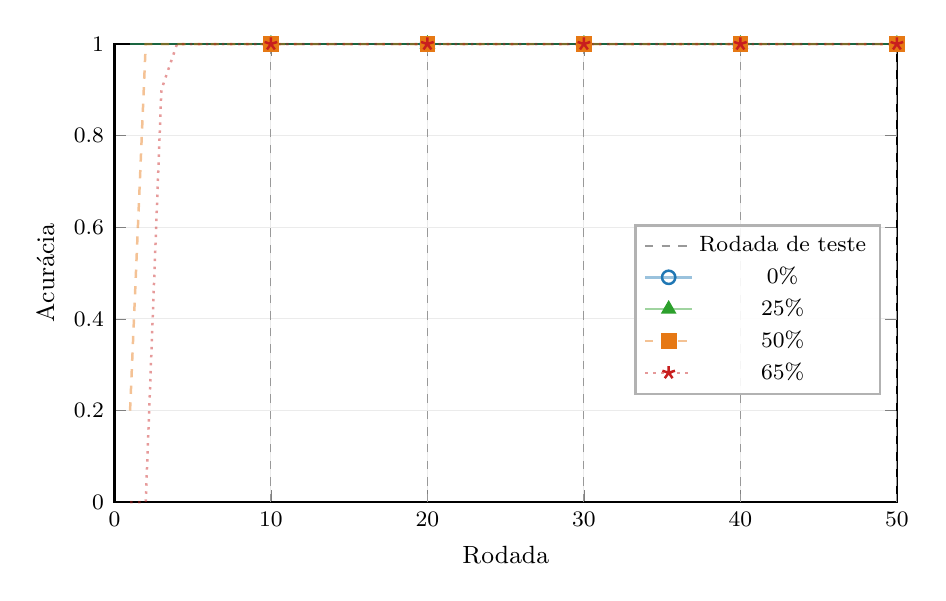
\begin{tikzpicture}
    \begin{axis}[
      teste fixo,
      width=0.95\textwidth,
      height=7.4cm,
      ylabel={Acurácia},
      legend style={
        at={(0.98,0.42)},
        anchor=east,
        font=\footnotesize,
        fill=white,
        fill opacity=0.9,
        text opacity=1,
        draw=black!30
      }
    ]
\draw[black!40, dashed, thin] (axis cs:10,\pgfkeysvalueof{/pgfplots/ymin}) -- (axis cs:10,\pgfkeysvalueof{/pgfplots/ymax});
\draw[black!40, dashed, thin] (axis cs:20,\pgfkeysvalueof{/pgfplots/ymin}) -- (axis cs:20,\pgfkeysvalueof{/pgfplots/ymax});
\draw[black!40, dashed, thin] (axis cs:30,\pgfkeysvalueof{/pgfplots/ymin}) -- (axis cs:30,\pgfkeysvalueof{/pgfplots/ymax});
\draw[black!40, dashed, thin] (axis cs:40,\pgfkeysvalueof{/pgfplots/ymin}) -- (axis cs:40,\pgfkeysvalueof{/pgfplots/ymax});
\draw[black!40, dashed, thin] (axis cs:50,\pgfkeysvalueof{/pgfplots/ymin}) -- (axis cs:50,\pgfkeysvalueof{/pgfplots/ymax});
\addlegendimage{black!40, dashed}
\addlegendentry{Rodada de teste}
\addplot[serieZero, solid, mark=o, opacity=0.45, mark repeat=10, mark phase=10, mark size=2.4pt, mark options={solid, opacity=1}] coordinates {(1,1.000) (2,1.000) (3,1.000) (4,1.000) (5,1.000) (6,1.000) (7,1.000) (8,1.000) (9,1.000) (10,1.000) (11,1.000) (12,1.000) (13,1.000) (14,1.000) (15,1.000) (16,1.000) (17,1.000) (18,1.000) (19,1.000) (20,1.000) (21,1.000) (22,1.000) (23,1.000) (24,1.000) (25,1.000) (26,1.000) (27,1.000) (28,1.000) (29,1.000) (30,1.000) (31,1.000) (32,1.000) (33,1.000) (34,1.000) (35,1.000) (36,1.000) (37,1.000) (38,1.000) (39,1.000) (40,1.000) (41,1.000) (42,1.000) (43,1.000) (44,1.000) (45,1.000) (46,1.000) (47,1.000) (48,1.000) (49,1.000) (50,1.000)};
\addlegendentry{0\%}
\addplot[serieVinte, solid, mark=triangle*, opacity=0.45, mark repeat=10, mark phase=10, mark size=2.4pt, mark options={solid, opacity=1}] coordinates {(1,1.000) (2,1.000) (3,1.000) (4,1.000) (5,1.000) (6,1.000) (7,1.000) (8,1.000) (9,1.000) (10,1.000) (11,1.000) (12,1.000) (13,1.000) (14,1.000) (15,1.000) (16,1.000) (17,1.000) (18,1.000) (19,1.000) (20,1.000) (21,1.000) (22,1.000) (23,1.000) (24,1.000) (25,1.000) (26,1.000) (27,1.000) (28,1.000) (29,1.000) (30,1.000) (31,1.000) (32,1.000) (33,1.000) (34,1.000) (35,1.000) (36,1.000) (37,1.000) (38,1.000) (39,1.000) (40,1.000) (41,1.000) (42,1.000) (43,1.000) (44,1.000) (45,1.000) (46,1.000) (47,1.000) (48,1.000) (49,1.000) (50,1.000)};
\addlegendentry{25\%}
\addplot[serieCinquenta, dashed, mark=square*, opacity=0.45, mark repeat=10, mark phase=10, mark size=2.4pt, mark options={solid, opacity=1}] coordinates {(1,0.200) (2,1.000) (3,1.000) (4,1.000) (5,1.000) (6,1.000) (7,1.000) (8,1.000) (9,1.000) (10,1.000) (11,1.000) (12,1.000) (13,1.000) (14,1.000) (15,1.000) (16,1.000) (17,1.000) (18,1.000) (19,1.000) (20,1.000) (21,1.000) (22,1.000) (23,1.000) (24,1.000) (25,1.000) (26,1.000) (27,1.000) (28,1.000) (29,1.000) (30,1.000) (31,1.000) (32,1.000) (33,1.000) (34,1.000) (35,1.000) (36,1.000) (37,1.000) (38,1.000) (39,1.000) (40,1.000) (41,1.000) (42,1.000) (43,1.000) (44,1.000) (45,1.000) (46,1.000) (47,1.000) (48,1.000) (49,1.000) (50,1.000)};
\addlegendentry{50\%}
\addplot[serieSessenta, dotted, mark=star, opacity=0.45, mark repeat=10, mark phase=10, mark size=2.4pt, mark options={solid, opacity=1}] coordinates {(1,0.000) (2,0.000) (3,0.900) (4,1.000) (5,1.000) (6,1.000) (7,1.000) (8,1.000) (9,1.000) (10,1.000) (11,1.000) (12,1.000) (13,1.000) (14,1.000) (15,1.000) (16,1.000) (17,1.000) (18,1.000) (19,1.000) (20,1.000) (21,1.000) (22,1.000) (23,1.000) (24,1.000) (25,1.000) (26,1.000) (27,1.000) (28,1.000) (29,1.000) (30,1.000) (31,1.000) (32,1.000) (33,1.000) (34,1.000) (35,1.000) (36,1.000) (37,1.000) (38,1.000) (39,1.000) (40,1.000) (41,1.000) (42,1.000) (43,1.000) (44,1.000) (45,1.000) (46,1.000) (47,1.000) (48,1.000) (49,1.000) (50,1.000)};
\addlegendentry{65\%}
    \end{axis}
  \end{tikzpicture}
  \caption{Acurácia do consenso ponderado por rodada, com conluio, 20 nós e EMA. Média de 10 sementes. A curva de 0\% é o cenário sem nós maliciosos, em que não há conluio. As linhas verticais marcam os testes das rodadas 10, 20, 30, 40 e 50.}
  \label{fig:acuracia-conluio}
\end{figure}


\begin{figure}[htbp]
  \centering
  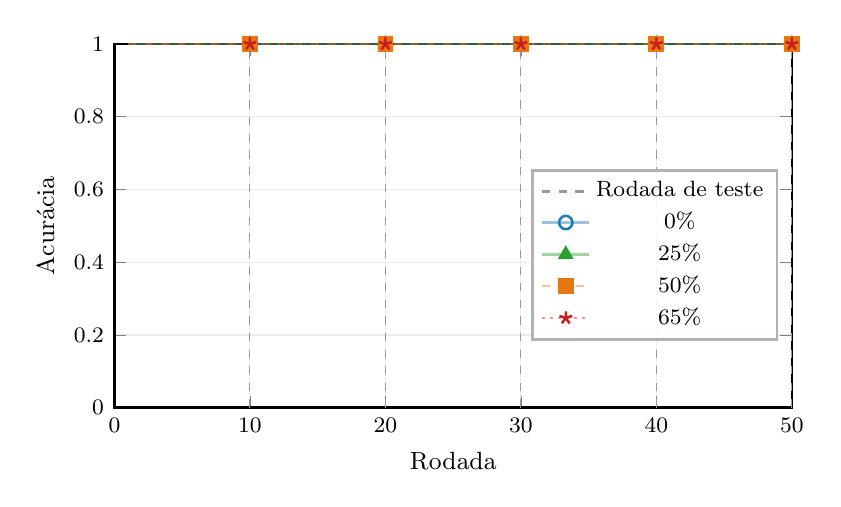
\begin{tikzpicture}
    \begin{axis}[
      teste fixo,
      width=0.84\textwidth,
      height=6.2cm,
      ylabel={Acurácia},
      legend style={
        at={(0.98,0.42)},
        anchor=east,
        font=\footnotesize,
        fill=white,
        fill opacity=0.9,
        text opacity=1,
        draw=black!30
      }
    ]
\draw[black!40, dashed, thin] (axis cs:10,\pgfkeysvalueof{/pgfplots/ymin}) -- (axis cs:10,\pgfkeysvalueof{/pgfplots/ymax});
\draw[black!40, dashed, thin] (axis cs:20,\pgfkeysvalueof{/pgfplots/ymin}) -- (axis cs:20,\pgfkeysvalueof{/pgfplots/ymax});
\draw[black!40, dashed, thin] (axis cs:30,\pgfkeysvalueof{/pgfplots/ymin}) -- (axis cs:30,\pgfkeysvalueof{/pgfplots/ymax});
\draw[black!40, dashed, thin] (axis cs:40,\pgfkeysvalueof{/pgfplots/ymin}) -- (axis cs:40,\pgfkeysvalueof{/pgfplots/ymax});
\draw[black!40, dashed, thin] (axis cs:50,\pgfkeysvalueof{/pgfplots/ymin}) -- (axis cs:50,\pgfkeysvalueof{/pgfplots/ymax});
\addlegendimage{black!40, dashed}
\addlegendentry{Rodada de teste}
\addplot[serieZero, solid, mark=o, opacity=0.45, mark repeat=10, mark phase=10, mark size=2.4pt, mark options={solid, opacity=1}] coordinates {(1,1.000) (2,1.000) (3,1.000) (4,1.000) (5,1.000) (6,1.000) (7,1.000) (8,1.000) (9,1.000) (10,1.000) (11,1.000) (12,1.000) (13,1.000) (14,1.000) (15,1.000) (16,1.000) (17,1.000) (18,1.000) (19,1.000) (20,1.000) (21,1.000) (22,1.000) (23,1.000) (24,1.000) (25,1.000) (26,1.000) (27,1.000) (28,1.000) (29,1.000) (30,1.000) (31,1.000) (32,1.000) (33,1.000) (34,1.000) (35,1.000) (36,1.000) (37,1.000) (38,1.000) (39,1.000) (40,1.000) (41,1.000) (42,1.000) (43,1.000) (44,1.000) (45,1.000) (46,1.000) (47,1.000) (48,1.000) (49,1.000) (50,1.000)};
\addlegendentry{0\%}
\addplot[serieVinte, solid, mark=triangle*, opacity=0.45, mark repeat=10, mark phase=10, mark size=2.4pt, mark options={solid, opacity=1}] coordinates {(1,1.000) (2,1.000) (3,1.000) (4,1.000) (5,1.000) (6,1.000) (7,1.000) (8,1.000) (9,1.000) (10,1.000) (11,1.000) (12,1.000) (13,1.000) (14,1.000) (15,1.000) (16,1.000) (17,1.000) (18,1.000) (19,1.000) (20,1.000) (21,1.000) (22,1.000) (23,1.000) (24,1.000) (25,1.000) (26,1.000) (27,1.000) (28,1.000) (29,1.000) (30,1.000) (31,1.000) (32,1.000) (33,1.000) (34,1.000) (35,1.000) (36,1.000) (37,1.000) (38,1.000) (39,1.000) (40,1.000) (41,1.000) (42,1.000) (43,1.000) (44,1.000) (45,1.000) (46,1.000) (47,1.000) (48,1.000) (49,1.000) (50,1.000)};
\addlegendentry{25\%}
\addplot[serieCinquenta, dashed, mark=square*, opacity=0.45, mark repeat=10, mark phase=10, mark size=2.4pt, mark options={solid, opacity=1}] coordinates {(1,1.000) (2,1.000) (3,1.000) (4,1.000) (5,1.000) (6,1.000) (7,1.000) (8,1.000) (9,1.000) (10,1.000) (11,1.000) (12,1.000) (13,1.000) (14,1.000) (15,1.000) (16,1.000) (17,1.000) (18,1.000) (19,1.000) (20,1.000) (21,1.000) (22,1.000) (23,1.000) (24,1.000) (25,1.000) (26,1.000) (27,1.000) (28,1.000) (29,1.000) (30,1.000) (31,1.000) (32,1.000) (33,1.000) (34,1.000) (35,1.000) (36,1.000) (37,1.000) (38,1.000) (39,1.000) (40,1.000) (41,1.000) (42,1.000) (43,1.000) (44,1.000) (45,1.000) (46,1.000) (47,1.000) (48,1.000) (49,1.000) (50,1.000)};
\addlegendentry{50\%}
\addplot[serieSessenta, dotted, mark=star, opacity=0.45, mark repeat=10, mark phase=10, mark size=2.4pt, mark options={solid, opacity=1}] coordinates {(1,1.000) (2,1.000) (3,1.000) (4,1.000) (5,1.000) (6,1.000) (7,1.000) (8,1.000) (9,1.000) (10,1.000) (11,1.000) (12,1.000) (13,1.000) (14,1.000) (15,1.000) (16,1.000) (17,1.000) (18,1.000) (19,1.000) (20,1.000) (21,1.000) (22,1.000) (23,1.000) (24,1.000) (25,1.000) (26,1.000) (27,1.000) (28,1.000) (29,1.000) (30,1.000) (31,1.000) (32,1.000) (33,1.000) (34,1.000) (35,1.000) (36,1.000) (37,1.000) (38,1.000) (39,1.000) (40,1.000) (41,1.000) (42,1.000) (43,1.000) (44,1.000) (45,1.000) (46,1.000) (47,1.000) (48,1.000) (49,1.000) (50,1.000)};
\addlegendentry{65\%}
    \end{axis}
  \end{tikzpicture}
  \caption{Acurácia do consenso ponderado por rodada, sem conluio, 20 nós e EMA. Média de 10 sementes. Sem um bloco único de respostas erradas, as curvas ficam sobrepostas; a transparência deixa essa coincidência visível.}
  \label{fig:acuracia-sem-conluio}
\end{figure}


\begin{figure}[htbp]
  \centering
  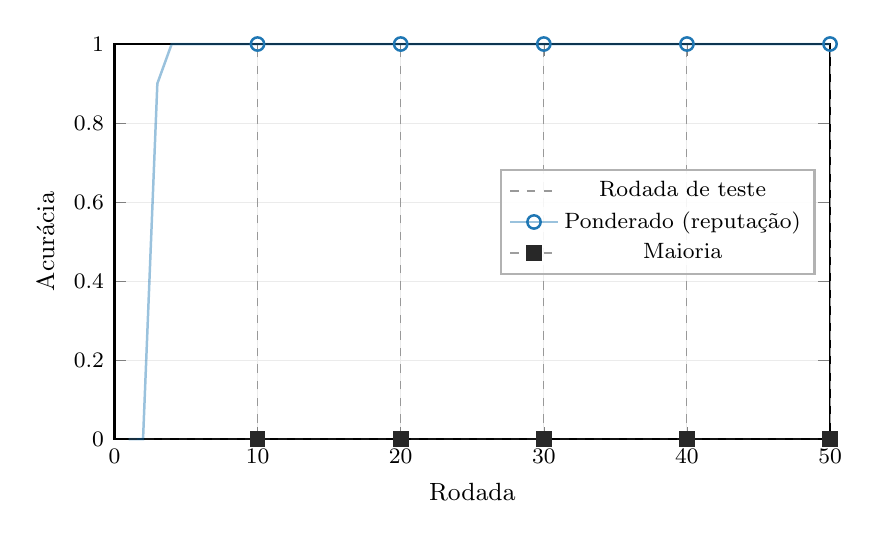
\begin{tikzpicture}
    \begin{axis}[
      teste fixo,
      width=0.88\textwidth,
      height=6.6cm,
      ylabel={Acurácia},
      legend style={
        at={(0.98,0.55)},
        anchor=east,
        font=\footnotesize,
        fill=white,
        fill opacity=0.9,
        text opacity=1,
        draw=black!30
      }
    ]
\draw[black!40, dashed, thin] (axis cs:10,\pgfkeysvalueof{/pgfplots/ymin}) -- (axis cs:10,\pgfkeysvalueof{/pgfplots/ymax});
\draw[black!40, dashed, thin] (axis cs:20,\pgfkeysvalueof{/pgfplots/ymin}) -- (axis cs:20,\pgfkeysvalueof{/pgfplots/ymax});
\draw[black!40, dashed, thin] (axis cs:30,\pgfkeysvalueof{/pgfplots/ymin}) -- (axis cs:30,\pgfkeysvalueof{/pgfplots/ymax});
\draw[black!40, dashed, thin] (axis cs:40,\pgfkeysvalueof{/pgfplots/ymin}) -- (axis cs:40,\pgfkeysvalueof{/pgfplots/ymax});
\draw[black!40, dashed, thin] (axis cs:50,\pgfkeysvalueof{/pgfplots/ymin}) -- (axis cs:50,\pgfkeysvalueof{/pgfplots/ymax});
\addlegendimage{black!40, dashed}
\addlegendentry{Rodada de teste}
\addplot[serieZero, solid, mark=o, opacity=0.45, mark repeat=10, mark phase=10, mark size=2.4pt, mark options={solid, opacity=1}] coordinates {(1,0.000) (2,0.000) (3,0.900) (4,1.000) (5,1.000) (6,1.000) (7,1.000) (8,1.000) (9,1.000) (10,1.000) (11,1.000) (12,1.000) (13,1.000) (14,1.000) (15,1.000) (16,1.000) (17,1.000) (18,1.000) (19,1.000) (20,1.000) (21,1.000) (22,1.000) (23,1.000) (24,1.000) (25,1.000) (26,1.000) (27,1.000) (28,1.000) (29,1.000) (30,1.000) (31,1.000) (32,1.000) (33,1.000) (34,1.000) (35,1.000) (36,1.000) (37,1.000) (38,1.000) (39,1.000) (40,1.000) (41,1.000) (42,1.000) (43,1.000) (44,1.000) (45,1.000) (46,1.000) (47,1.000) (48,1.000) (49,1.000) (50,1.000)};
\addlegendentry{Ponderado (reputação)}
\addplot[serieMaioria, dashed, mark=square*, opacity=0.45, mark repeat=10, mark phase=10, mark size=2.4pt, mark options={solid, opacity=1}] coordinates {(1,0.000) (2,0.000) (3,0.000) (4,0.000) (5,0.000) (6,0.000) (7,0.000) (8,0.000) (9,0.000) (10,0.000) (11,0.000) (12,0.000) (13,0.000) (14,0.000) (15,0.000) (16,0.000) (17,0.000) (18,0.000) (19,0.000) (20,0.000) (21,0.000) (22,0.000) (23,0.000) (24,0.000) (25,0.000) (26,0.000) (27,0.000) (28,0.000) (29,0.000) (30,0.000) (31,0.000) (32,0.000) (33,0.000) (34,0.000) (35,0.000) (36,0.000) (37,0.000) (38,0.000) (39,0.000) (40,0.000) (41,0.000) (42,0.000) (43,0.000) (44,0.000) (45,0.000) (46,0.000) (47,0.000) (48,0.000) (49,0.000) (50,0.000)};
\addlegendentry{Maioria}
    \end{axis}
  \end{tikzpicture}
  \caption{Consenso ponderado e maioria ao longo das rodadas, com 65\% de nós maliciosos em conluio (13 de 20), EMA, média de 10 sementes.}
  \label{fig:ponderado-vs-maioria-65}
\end{figure}


\begin{figure}[htbp]
  \centering
  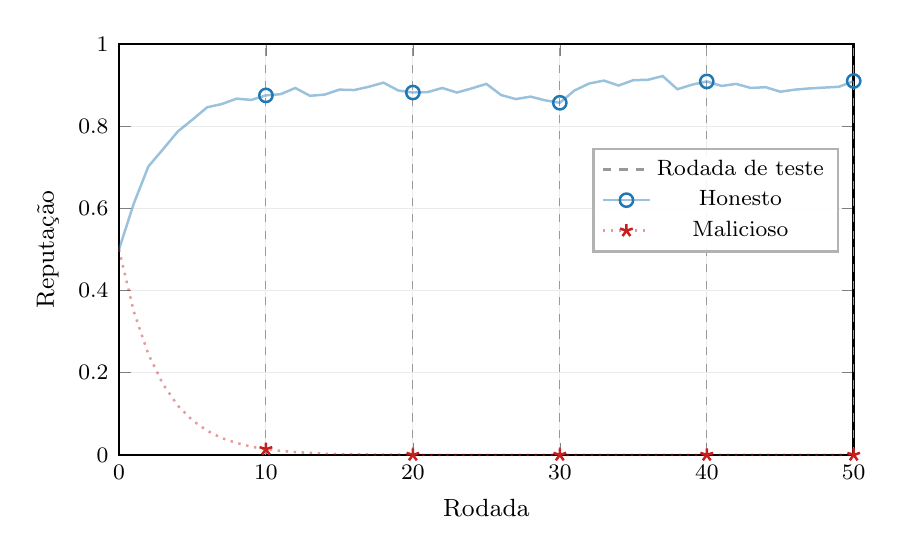
\begin{tikzpicture}
    \begin{axis}[
      teste fixo,
      width=0.90\textwidth,
      height=6.8cm,
      ylabel={Reputação},
      legend style={
        at={(0.98,0.62)},
        anchor=east,
        font=\footnotesize,
        fill=white,
        fill opacity=0.9,
        text opacity=1,
        draw=black!30
      }
    ]
\draw[black!40, dashed, thin] (axis cs:10,\pgfkeysvalueof{/pgfplots/ymin}) -- (axis cs:10,\pgfkeysvalueof{/pgfplots/ymax});
\draw[black!40, dashed, thin] (axis cs:20,\pgfkeysvalueof{/pgfplots/ymin}) -- (axis cs:20,\pgfkeysvalueof{/pgfplots/ymax});
\draw[black!40, dashed, thin] (axis cs:30,\pgfkeysvalueof{/pgfplots/ymin}) -- (axis cs:30,\pgfkeysvalueof{/pgfplots/ymax});
\draw[black!40, dashed, thin] (axis cs:40,\pgfkeysvalueof{/pgfplots/ymin}) -- (axis cs:40,\pgfkeysvalueof{/pgfplots/ymax});
\draw[black!40, dashed, thin] (axis cs:50,\pgfkeysvalueof{/pgfplots/ymin}) -- (axis cs:50,\pgfkeysvalueof{/pgfplots/ymax});
\addlegendimage{black!40, dashed}
\addlegendentry{Rodada de teste}
\addplot[serieZero, solid, mark=o, opacity=0.45, mark repeat=10, mark phase=11, mark size=2.4pt, mark options={solid, opacity=1}] coordinates {(0,0.500) (1,0.611) (2,0.702) (3,0.744) (4,0.787) (5,0.816) (6,0.846) (7,0.854) (8,0.867) (9,0.864) (10,0.875) (11,0.878) (12,0.893) (13,0.874) (14,0.877) (15,0.889) (16,0.888) (17,0.896) (18,0.906) (19,0.887) (20,0.882) (21,0.883) (22,0.893) (23,0.882) (24,0.892) (25,0.903) (26,0.876) (27,0.866) (28,0.872) (29,0.863) (30,0.857) (31,0.887) (32,0.904) (33,0.911) (34,0.899) (35,0.912) (36,0.913) (37,0.922) (38,0.890) (39,0.901) (40,0.909) (41,0.898) (42,0.903) (43,0.893) (44,0.895) (45,0.884) (46,0.889) (47,0.892) (48,0.894) (49,0.896) (50,0.910)};
\addlegendentry{Honesto}
\addplot[serieSessenta, dotted, mark=star, opacity=0.45, mark repeat=10, mark phase=11, mark size=2.4pt, mark options={solid, opacity=1}] coordinates {(0,0.500) (1,0.350) (2,0.245) (3,0.172) (4,0.120) (5,0.084) (6,0.059) (7,0.041) (8,0.029) (9,0.020) (10,0.014) (11,0.010) (12,0.007) (13,0.005) (14,0.003) (15,0.002) (16,0.002) (17,0.001) (18,0.001) (19,0.001) (20,0.000) (21,0.000) (22,0.000) (23,0.000) (24,0.000) (25,0.000) (26,0.000) (27,0.000) (28,0.000) (29,0.000) (30,0.000) (31,0.000) (32,0.000) (33,0.000) (34,0.000) (35,0.000) (36,0.000) (37,0.000) (38,0.000) (39,0.000) (40,0.000) (41,0.000) (42,0.000) (43,0.000) (44,0.000) (45,0.000) (46,0.000) (47,0.000) (48,0.000) (49,0.000) (50,0.000)};
\addlegendentry{Malicioso}
    \end{axis}
  \end{tikzpicture}
  \caption{Reputação média dos nós honestos e maliciosos com 65\% de maliciosos em conluio, 20 nós e EMA. A linha vermelha pontilhada é o perfil malicioso. Marcadores e linhas verticais nas rodadas de teste.}
  \label{fig:reputacao-65}
\end{figure}


\begin{figure}[htbp]
  \centering
  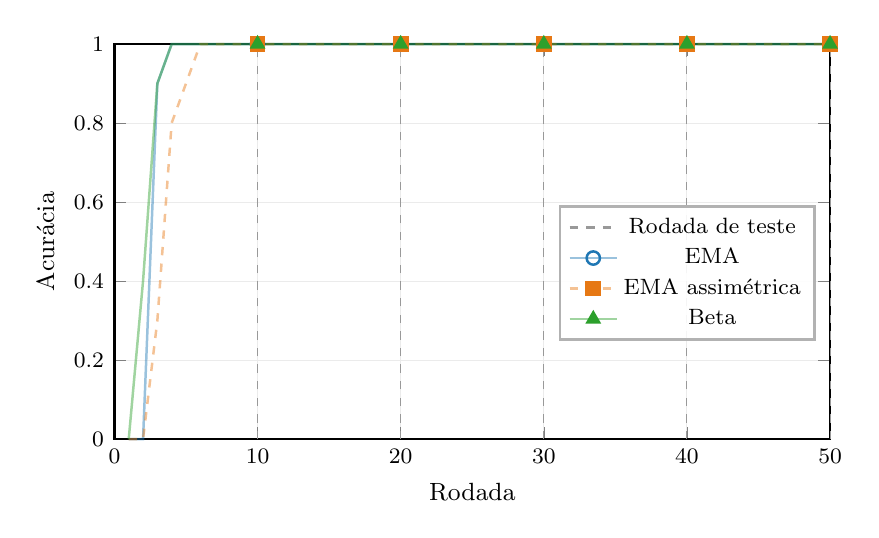
\begin{tikzpicture}
    \begin{axis}[
      teste fixo,
      width=0.88\textwidth,
      height=6.6cm,
      ylabel={Acurácia},
      legend style={
        at={(0.98,0.42)},
        anchor=east,
        font=\footnotesize,
        fill=white,
        fill opacity=0.9,
        text opacity=1,
        draw=black!30
      }
    ]
\draw[black!40, dashed, thin] (axis cs:10,\pgfkeysvalueof{/pgfplots/ymin}) -- (axis cs:10,\pgfkeysvalueof{/pgfplots/ymax});
\draw[black!40, dashed, thin] (axis cs:20,\pgfkeysvalueof{/pgfplots/ymin}) -- (axis cs:20,\pgfkeysvalueof{/pgfplots/ymax});
\draw[black!40, dashed, thin] (axis cs:30,\pgfkeysvalueof{/pgfplots/ymin}) -- (axis cs:30,\pgfkeysvalueof{/pgfplots/ymax});
\draw[black!40, dashed, thin] (axis cs:40,\pgfkeysvalueof{/pgfplots/ymin}) -- (axis cs:40,\pgfkeysvalueof{/pgfplots/ymax});
\draw[black!40, dashed, thin] (axis cs:50,\pgfkeysvalueof{/pgfplots/ymin}) -- (axis cs:50,\pgfkeysvalueof{/pgfplots/ymax});
\addlegendimage{black!40, dashed}
\addlegendentry{Rodada de teste}
\addplot[serieZero, solid, mark=o, opacity=0.45, mark repeat=10, mark phase=10, mark size=2.4pt, mark options={solid, opacity=1}] coordinates {(1,0.000) (2,0.000) (3,0.900) (4,1.000) (5,1.000) (6,1.000) (7,1.000) (8,1.000) (9,1.000) (10,1.000) (11,1.000) (12,1.000) (13,1.000) (14,1.000) (15,1.000) (16,1.000) (17,1.000) (18,1.000) (19,1.000) (20,1.000) (21,1.000) (22,1.000) (23,1.000) (24,1.000) (25,1.000) (26,1.000) (27,1.000) (28,1.000) (29,1.000) (30,1.000) (31,1.000) (32,1.000) (33,1.000) (34,1.000) (35,1.000) (36,1.000) (37,1.000) (38,1.000) (39,1.000) (40,1.000) (41,1.000) (42,1.000) (43,1.000) (44,1.000) (45,1.000) (46,1.000) (47,1.000) (48,1.000) (49,1.000) (50,1.000)};
\addlegendentry{EMA}
\addplot[serieCinquenta, dashed, mark=square*, opacity=0.45, mark repeat=10, mark phase=10, mark size=2.4pt, mark options={solid, opacity=1}] coordinates {(1,0.000) (2,0.000) (3,0.300) (4,0.800) (5,0.900) (6,1.000) (7,1.000) (8,1.000) (9,1.000) (10,1.000) (11,1.000) (12,1.000) (13,1.000) (14,1.000) (15,1.000) (16,1.000) (17,1.000) (18,1.000) (19,1.000) (20,1.000) (21,1.000) (22,1.000) (23,1.000) (24,1.000) (25,1.000) (26,1.000) (27,1.000) (28,1.000) (29,1.000) (30,1.000) (31,1.000) (32,1.000) (33,1.000) (34,1.000) (35,1.000) (36,1.000) (37,1.000) (38,1.000) (39,1.000) (40,1.000) (41,1.000) (42,1.000) (43,1.000) (44,1.000) (45,1.000) (46,1.000) (47,1.000) (48,1.000) (49,1.000) (50,1.000)};
\addlegendentry{EMA assimétrica}
\addplot[serieVinte, solid, mark=triangle*, opacity=0.45, mark repeat=10, mark phase=10, mark size=2.4pt, mark options={solid, opacity=1}] coordinates {(1,0.000) (2,0.400) (3,0.900) (4,1.000) (5,1.000) (6,1.000) (7,1.000) (8,1.000) (9,1.000) (10,1.000) (11,1.000) (12,1.000) (13,1.000) (14,1.000) (15,1.000) (16,1.000) (17,1.000) (18,1.000) (19,1.000) (20,1.000) (21,1.000) (22,1.000) (23,1.000) (24,1.000) (25,1.000) (26,1.000) (27,1.000) (28,1.000) (29,1.000) (30,1.000) (31,1.000) (32,1.000) (33,1.000) (34,1.000) (35,1.000) (36,1.000) (37,1.000) (38,1.000) (39,1.000) (40,1.000) (41,1.000) (42,1.000) (43,1.000) (44,1.000) (45,1.000) (46,1.000) (47,1.000) (48,1.000) (49,1.000) (50,1.000)};
\addlegendentry{Beta}
    \end{axis}
  \end{tikzpicture}
  \caption{Acurácia do consenso ponderado por mecanismo, com 65\% de nós maliciosos em conluio e 20 nós. Média de 10 sementes.}
  \label{fig:mecanismos-65}
\end{figure}

